% slides.tex
\documentclass[20pt]{beamer}
\usepackage{listings}
\usepackage[utf8]{inputenc}
\usepackage{color}
\usepackage{graphicx}

\usetheme{default}
\usecolortheme{dove}
\useoutertheme{default}

% Slightly smaller title
\setbeamerfont{frametitle}{size=\large}
\setbeamerfont{verb}{size=\small}

% lst settings
\lstset{
    language=Haskell,
    basicstyle=\small,
    gobble=4
}

\newcommand{\vspaced}{
    \vspace{5mm}
}

\begin{document}

\title{The Text library}
\subtitle{8th GhentFPG meeting}
\author{Jasper Van der Jeugt}
\date{May 30, 2011}

\begin{frame}[plain]
    \titlepage
\end{frame}

% Introduction
% ------------

\begin{frame}{Hello!}
    My name is Jasper \\
    Student at UGent \\
    I write Haskell \\
    GhentFPG \\
    \texttt{@jaspervdj} \\
    \texttt{jaspervdj.be}
    \begin{picture}(0.0, 0.0)
    \put(40.0, -15.0){
        
\includegraphics[width=0.5\textwidth]{../2011-functionalpx-blaze-html/images/hat.pdf}}
    \end{picture}
\end{frame}

\begin{frame}{Overview}
    Herp derp
\end{frame}

% Strictness analysis
% -------------------

\begin{frame}{Strictness analysis}
    Haskell has lazy evaluation as default
\end{frame}

\begin{frame}{Strictness analysis}
    Lazy evaluation leads to more composable code \\
    \vspaced
    Disadvantage: too much laziness
\end{frame}

\begin{frame}[fragile]{Strictness analysis}
    A function can be strict in it's arguments
    \vspaced
    \begin{lstlisting}
    null :: [a] -> Bool
    null [] = True
    null _  = False
    \end{lstlisting}
\end{frame}

\begin{frame}[fragile]{Strictness analysis}
    \begin{lstlisting}
    hello :: String -> String
    hello name =
      "Hello, " ++ name ++ "!"
    \end{lstlisting}
\end{frame}

\begin{frame}[fragile]{Strictness analysis}
    \begin{lstlisting}
    quadr :: Floating a
          => a -> a -> a -> a -> a
    quadr a b c x =
      a * x ^ 2 + b * x + c
    \end{lstlisting}
\end{frame}

\begin{frame}[fragile]{Strictness analysis}
    \begin{lstlisting}
    if' :: Bool -> a -> a -> a
    if' True  x _ = x
    if' False _ y = y
    \end{lstlisting}
\end{frame}

\begin{frame}[fragile]{Strictness analysis}
    \begin{lstlisting}
    maybe ::
      b -> (a -> b) -> Maybe a -> b
    maybe d _ Nothing  = d
    maybe _ f (Just x) = f x
    \end{lstlisting}
\end{frame}

\begin{frame}[fragile]{Strictness analysis}
    Functions can easily be made strict \\
    \vspaced
    \begin{lstlisting}
    seq :: a -> b -> b
    \end{lstlisting}
\end{frame}

\begin{frame}[fragile]{Strictness analysis}
    \begin{lstlisting}
    quadr :: Floating a
          => a -> a -> a -> a -> a
    quadr a b c x =
      a `seq` b `seq` c `seq`
        a * x ^ 2 + b * x + c
    \end{lstlisting}
\end{frame}

\begin{frame}[fragile]{Strictness analysis}
    Useful syntactic sugar \\
    \vspaced
    \begin{lstlisting}
    {-# LANGUAGE BangPatterns #-}
    quadr :: Floating a
          => a -> a -> a -> a -> a
    quadr !a !b !c x =
      a * x ^ 2 + b * x + c
    \end{lstlisting}
\end{frame}

% Unboxed types
% -------------

% Benchmarking pitfalls
% ---------------------

\begin{frame}{Benchmarking pitfalls}
    Haskell is a lazy language \\
    This makes benchmarking hard
\end{frame}

\begin{frame}{Benchmarking pitfalls}
    Two types of benchmarks: \\
    Functions and programs \\
    \vspaced
    (we focus on the former)
\end{frame}

\begin{frame}[fragile]{Benchmarking pitfalls}
    Benchmarking some function

    \begin{lstlisting}
    f :: Int -> Int
    \end{lstlisting}
\end{frame}

\begin{frame}[fragile]{Benchmarking pitfalls}
    In e.g. Python
    \vspaced
    \begin{lstlisting}
    total = 0
    for i in range(100):
        start = time.time()
        f()
        end = time.time()
        total += (end - start) / 100
    \end{lstlisting}
\end{frame}

\begin{frame}[fragile]{Benchmarking pitfalls}
    In Haskell?
    \vspaced
    \begin{lstlisting}
    replicateM 100 $ do
        start <- getTime
        let y = f x
        end <- y `seq` getTime
    \end{lstlisting}
    \vspaced
    This is pretty hard to get right
\end{frame}

\begin{frame}{Benchmarking pitfalls}
    Conclusion? \\
    \vspaced
    \textbf{Never write your own benchmarking code}
\end{frame}

\begin{frame}{Benchmarking pitfalls}
    \textbf{Criterion} \\
    \vspaced
    By Bryan O'Sullivan
\end{frame}

\begin{frame}[fragile]{Benchmarking pitfalls}
    Criterion \\
    \vspaced
    \begin{lstlisting}
    bench "f" $ nf   f x
    bench "g" $ whnf g x
    \end{lstlisting}
\end{frame}

\begin{frame}[fragile]{Benchmarking pitfalls}
    \texttt{Eq} for string types \\
    \vspaced
    \begin{lstlisting}
    whnf (== T.init t
        `T.snoc` '\xfffd') t

    whnf (== BL.init bl
        `BL.snoc` '\xfffd') bl
    \end{lstlisting}
\end{frame}

\begin{frame}{Benchmarking pitfalls}
    But \texttt{ByteString.Lazy} \\
    is a little faster \\
    \vspaced
    \texttt{Text}: 2.489305 us
    \texttt{ByteString.Lazy}: 39.29312 \textbf{ns}
\end{frame}

\begin{frame}[fragile]{Benchmarking pitfalls}
    Digging into the code... \\
    \vspaced
    \begin{lstlisting}
    eq (Chunk a as) (Chunk b bs) =
      case compare (S.length a)
                   (S.length b) of
        ...
        EQ -> a == b && eq as bs
        ...
    \end{lstlisting}
\end{frame}

\begin{frame}[fragile]{Benchmarking pitfalls}
    Digging further... \\
    \vspaced
    \begin{lstlisting}
    eq a@(PS p s l) b@(PS p' s' l')
       -- short cut on length
       | l /= l'            = False
       -- short cut for same string
       | p == p' && s == s' = True
       | ...
    \end{lstlisting}
\end{frame}

\begin{frame}{Benchmarking pitfalls}
    Conclusion? \\
    \vspaced
    \textbf{Libraries can be smarter than you think they are, make sure you know
    whay you are benchmarking!}
\end{frame}

\begin{frame}[fragile]{Benchmarking pitfalls}
    Benchmarking IO \\
    \vspaced
    \begin{lstlisting}
    bench "HtmlCombinator" $ do
      putStr "Content-Type: ..."
      ...
      putStr "<table>"
      putStr $ toLazyText $
        makeTable 20000
      putStr "</table>"
    \end{lstlisting}
\end{frame}

\begin{frame}[fragile]{Benchmarking pitfalls}
    This looks suspicious \\
    \vspaced
    \begin{lstlisting}
    benchmarking HtmlCombinator
    collecting 100 samples (...)
        estimated 30.80161 s
    mean: 107.6378 ms (...)
    \end{lstlisting}
    \vspaced
    $100 * 100ms \neq 30s$
\end{frame}

\begin{frame}{Benchmarking pitfalls}
    \begin{center}
    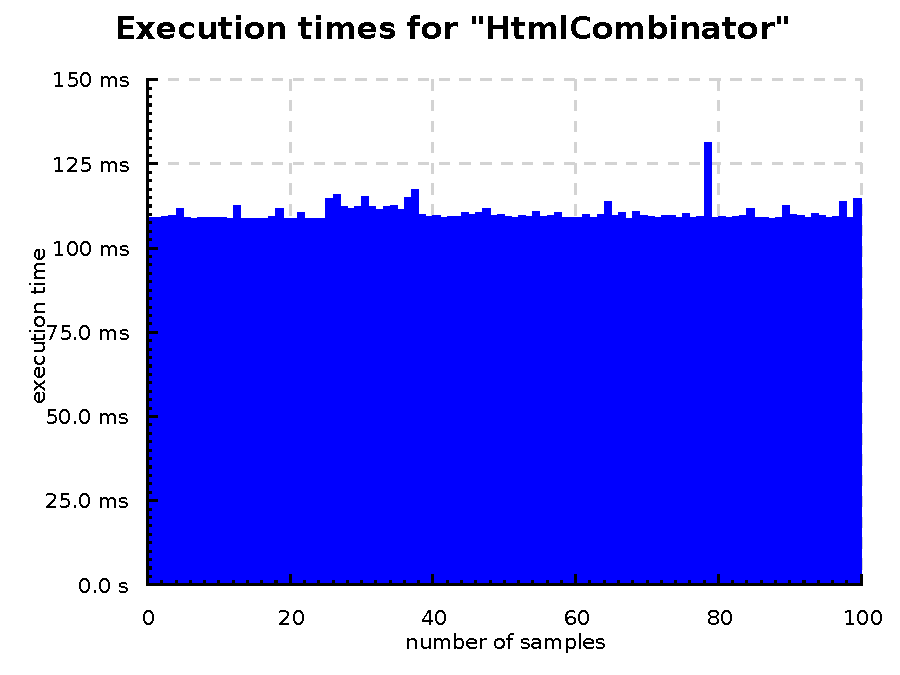
\includegraphics[width=0.9\textwidth]{images/htmlcombinator.pdf}
    \end{center}
\end{frame}

\begin{frame}[fragile]{Benchmarking pitfalls}
    Where is the issue? \\
    \vspaced
    \begin{lstlisting}
    bench "HtmlCombinator" $ do
      putStr "Content-Type: ..."
      ...
      putStr "<table>"
      putStr $ toLazyText $
        makeTable 20000
      putStr "</table>"
    \end{lstlisting}
\end{frame}

\begin{frame}[fragile]{Benchmarking pitfalls}
    \begin{lstlisting}
    putStr . toLazyText .
        makeTable =<< rows
    ...
    where
      rows :: IO Int
      rows = return 20000
      {-# NOINLINE rows #-}
    \end{lstlisting}
\end{frame}

\begin{frame}{Benchmarking pitfalls}
    Conclusion? \\
    \vspaced
    \textbf{GHC is pretty smart as well}
\end{frame}

% GHC Core
% --------

\end{document}
